\documentclass[a4paper]{article}

\usepackage[utf8]{inputenc}
\usepackage[T1]{fontenc}
\usepackage[frenchb]{babel}
\usepackage{colortbl}
\usepackage{graphicx}
\usepackage{moresize}
\usepackage{anyfontsize}
\usepackage{hyperref}
\usepackage{longtable}
\usepackage[table]{xcolor}
\usepackage{tabularx}
\usepackage{pdfpages}
\usepackage{pdflscape}
\usepackage{lastpage}
\usepackage{array}
 \usepackage{float}
\usepackage{caption}
\usepackage{wrapfig}

% Definition des pages
\usepackage[left=3cm,right=3cm,top=3cm,bottom=3cm]{geometry}

% En-tete de page
\usepackage{fancyhdr}
\pagestyle{fancy}

% Lien hypertexte
\usepackage{hyperref}
\hypersetup{
  hidelinks,
  backref=true,
  pagebackref=true,
  hyperindex=true,
  colorlinks=false,
  breaklinks=true,
  urlcolor=ocre,
  bookmarks=true,
  bookmarksopen=false,
  pdftitle={Compte Rendu JEE},
  pdfauthor={Yohann HENRY - Jérémie PANTIN}
}

\definecolor{purp}{RGB}{110, 40, 150}
\definecolor{grisC}{RGB}{245, 245, 245}
\definecolor{grisF}{RGB}{224, 224, 224}
\definecolor{grisP}{RGB}{136, 136, 136}
\definecolor{ocre}{RGB}{51,102,0}

\makeatletter
\renewcommand{\@seccntformat}[1]{\llap{\textcolor{purp}{\csname the#1\endcsname}\hspace{1em}}}                    
\renewcommand{\section}{\@startsection{section}{1}{\z@}
{-4ex \@plus -1ex \@minus -.4ex}
{1ex \@plus.2ex }
{\normalfont\large\sffamily\bfseries}}
\renewcommand{\subsection}{\@startsection {subsection}{2}{\z@}
{-3ex \@plus -0.1ex \@minus -.4ex}
{0.5ex \@plus.2ex }
{\normalfont\sffamily\bfseries}}
\renewcommand{\subsubsection}{\@startsection {subsubsection}{3}{\z@}
{-2ex \@plus -0.1ex \@minus -.2ex}
{.2ex \@plus.2ex }
{\normalfont\small\sffamily\bfseries}}                        
\renewcommand\paragraph{\@startsection{paragraph}{4}{\z@}
{-2ex \@plus-.2ex \@minus .2ex}
{.1ex}
{\normalfont\small\sffamily\bfseries}}

\renewcommand\headrulewidth{1pt}
\fancyhead[L]{
\includegraphics[height=1cm]{univ.png}}
\fancyhead[C]{Compte Rendu\\ \color{grisP}\texttt{Projet JEE}}
\fancyfoot[C]{\texttt{\thepage/\pageref{LastPage}}}
\makeatletter
\newcommand{\resetHeadWidth}{\fancy@setoffs}
\makeatother


\renewcommand{\arraystretch}{1.5}

\begin{document}

\begin{titlepage}
	\begin{center}
		{\fontsize{22}{30}\selectfont Projet Architectures Orientées Services sous JEE\\Gestion de la Notification d'Effets Indésirables}\\[\baselineskip]
		\vspace*{10pt}
		{\Large\itshape 15/01/2017}\\
		\vfill
		\rule{0.6\textwidth}{0.4pt}\\[\baselineskip]
		\begin{table}[h]
			\centering
			\def\arraystretch{1.4}
			\begin{tabular}{ll|ll}
				Yohann & HENRY & Jérémie & PANTIN\\
			\end{tabular}
		\end{table}
	\end{center}
\end{titlepage}

\thispagestyle{empty}

\tableofcontents
\newpage
\setcounter{page}{1}
\vspace*{0.5cm}

\section{Introduction}
Internet est au coeur du monde d'aujourd'hui, il est alors logique pour les structures permettant son emploi de s'agrandir et se complexifier. Nous nous centrons ici sur une des solutions trouvées pour répondre au besoin d'applications toujours plus complètes : \texttt{JavaEE} (Java Entreprise Edition).

\section{Présentation}
\subsection{Contexte}
Il est demandé, dans ce projet, de développer une application web permettant de gérer des notifications d'effets indésirables survenus à la suite de l'utilisation d'un ou de plusieurs produits cosmétiques : \texttt{NotifCosmoEI}. Ces notifications peuvent être déclarées par plusieurs types d'utilisateurs :
\begin{itemize}
\item Utilisateur quelconque
\item Pharmacien
\item Association de consommateurs
\item Médecin
\item Laboratoire de cosmétiques
\end{itemize}

Dans le document ci-présent nous allons décrire la solution technique et justifier l'emploi de certaines orientations technologiques et techniques.

\subsection{JavaEE}
JavaEE est une plate-forme fortement orientée serveur ayant pour but de développer et exécuter des applications distribuées. Elle se compose de deux grandes parties : spécifications et serveur d'application(s). L'intérêt non moindre est de permettre à des entreprises, par exemple, de développer des serveurs d'applications conformes aux spécifications, sans avoir la nécessité de re-développer les services existants. Elle permet donc de faciliter le développement d'applications avec une Architecture Orientée Service, mais pas seulement.

\subsection{Spring}
\texttt{Spring} est un framework libre, conçu pour la création et la définition de l'infrastructure d'une application Java. Son but est de faciliter le développement et les tests. L'architecture de ce framework se compose de plus de 20 modules pouvant être utilisés en fonction de la demande :

\begin{figure}[h]
\centering
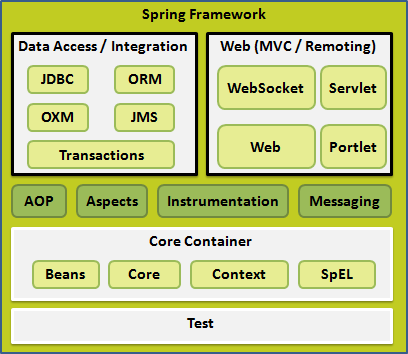
\includegraphics[scale=.7]{spring_architecture.png}
\caption{Architecture du Framework Spring}
\end{figure}

\newpage

\vspace*{0.5cm}

Nous emploierons donc ce framework afin de répondre à la demande de développer une Application Web. En effet, notre intention est de nous former à un framework grandement reconnu dans le monde et à prendre en main une technologie qui sera utiliser pendant le projet Annuel \texttt{TRAVEL}. Grâce à la formation aux AOS pendant les cours et les travaux pratiques du parcours M2GIL, nous allons présenter une démarche descriptive alliant méthodologie et respect des conventions apprises.

\section{Technologies}
Dans cette section sera présenté l'intégralité des technologies utilisées dans la réalisation de l'Application Web NotifCosmoEI. Y seront présentés également les versions utilisées de ces mêmes outils.

\subsection{Spring}

\begin{wrapfigure}{R}{0.15\textwidth}
\centering

\includegraphics[width=0.14\textwidth]{spring_logo.png}
\end{wrapfigure}

Comme décrit plus haut nous utiliserons le framework Spring afin de développer notre application. Ce framework permet la liaison avec de nombreux outils complémentaires qui ont étés également vus pendant le cursus de deuxième année de master.\\
Nous allons donc lister les principaux outils de développement utilisés par celui-ci et contextualiser leur emploi. Nous préciserons la version des outils en question également.

\subsubsection{Gradle}

\begin{wrapfigure}{R}{0.25\textwidth}
\centering

\includegraphics[width=0.24\textwidth]{gradle.png}
\end{wrapfigure}

Gradle est un moteur de production permettant de construire des projets Java. Il allie \texttt{Apache Maven} et \texttt{Apache Ant} pour en prendre uniquement leurs atouts. Ainsi il permet d'écrire des tâches de \texttt{build} dans un fichier \texttt{build} en utilisant le langage Groovy. Il est alors possible d'importer des tâches standards qui permettent de construire des programmes utilisant un ou plusieurs langages, Java dans notre cas.

\subsubsection{Maven 3}

\begin{wrapfigure}{R}{0.25\textwidth}
\centering

\includegraphics[width=0.24\textwidth]{maven.png}
\end{wrapfigure}

Apache Maven est un outil pour la gestion et l'automatisation de production des projets Java. Dans notre cas il sera employé pour ses conventions simples et efficaces, de part Gradle. En effet Maven impose une arborescence et une énumération des fichiers du projet selon le concept de Convention plutôt que configuration.

\subsubsection{Ant}
\begin{wrapfigure}{R}{0.15\textwidth}
\centering

\includegraphics[width=0.14\textwidth]{ant.png}
\end{wrapfigure}

Apache Ant est un logiciel visant à automatiser les opérations répétitives du développement de logiciel telles que la compilation, la génération de documents ou l'archivage. Utilisé par Gradle, sa tâche est de permettre la compilation, la génération, l'exécution et l'archivage sous forme distribuable (JAR, ...). Il faut savoir qu'il est très portable et flexible dans la description des tâches de construction.\\
C'est donc un indispensable pour fournir une application exécutable et portable.

\subsubsection{Spring Boot 1.4.2}
\begin{wrapfigure}{R}{0.15\textwidth}
\centering

\includegraphics[width=0.14\textwidth]{spring_boot.png}
\end{wrapfigure}

Spring Boot permet l'initialisation de nombreuses configurations automatisées :
\begin{itemize}
\item Initialisation du gestionnaire \texttt{DispatcherServlet} de Spring MVC
\item Configuration du filtre d'encodage au sein des requêtes clients
\item Configuration du routage des vues Spring afin de les situer et de les spécifier au sein du projet
\item Intégration de la location des ressources statiques (.css, .js, ...)
\item Configuration des ressources locales de bundles
\item Intégration de l'exécution Tomcat sur lequel l'application sera déployée
\end{itemize}

\vspace*{0.5cm}

\begin{itemize}
\item Configuration et création des gestion de pages d'erreurs (404, ...)
\end{itemize}

En outre, Spring Boot maintient l'intégralité de ces opérations pour nous.


\subsubsection{Spring Security}
\begin{wrapfigure}{R}{0.15\textwidth}
\centering

\includegraphics[width=0.14\textwidth]{spring_security.png}
\end{wrapfigure}

Spring Security offre des services de sécurité complets pour des applications basées sur JavaEE. Il s'intègre nativement à un projet Spring et permet de mettre notamment l'accent sur l'authentification et l'autorisation, entre autre le contrôle d'accès, et bien d'autres. Il est utilisé ici pour conserver un très haut niveau de sécurité au sein de la spécification des Servlet JavaEE et de la spécification des EJB.

\subsubsection{Spring MVC 1.0.1}
Spring propose l'élaboration d'une application sur l'architecture Model View Controller grâce à Spring MVC. Nous utiliserons donc ce dernier afin de respecter les conventions vues en cours et pratiqués lors des travaux pratiques. C'est également sur ce contexte que se basent nombre de solutions logicielles et web, auxquelles nous sommes sensibilisé depuis le début de notre cursus.

\subsection{Tomcat}
\begin{wrapfigure}{R}{0.15\textwidth}
\centering

\includegraphics[width=0.14\textwidth]{tomcat.png}
\end{wrapfigure}
Apache Tomcat est un conteneur web libre de servlets et JSP JavaEE. C'est un serveur HTTP, il répond alors parfaitement à la problématique du projet. Nous l'utiliserons et l'intégrerons directement en tant que serveur embarqué sur notre application par le biais de Spring (notamment par l'emploi du Spring Boot vu précédemment).

\subsection{Thymeleaf 2.1.2}
\begin{wrapfigure}{R}{0.15\textwidth}
\centering

\includegraphics[width=0.14\textwidth]{thymeleaf.png}
\end{wrapfigure}

Thymeleaf est un moteur de template utilisé dans un environnement web pour la génération de vue pour les applications web MVC. Nous justifions sa présence par sa simplicité d'utilisation et son extension facilité. De plus il répond aux besoins soulevés par le modèle MVC.\\
Un autre argument vient conforter ce choix, c'est sa grande popularité dans la communauté, nous permettant d'avoir accès à un large panel d'informations lors de problèmes rencontrés.

\subsection{PostgreSQL 9.1}
\begin{wrapfigure}{R}{0.15\textwidth}
\centering

\includegraphics[width=0.14\textwidth]{postgresql.png}
\end{wrapfigure}
Postegre SQL est un système de Gestion de Base de Données relationnelle et objet (SGBD). C'est un outil libre qui s'est forgé une réputation sur son comportement stable et ses possibilités de programmation étendues. Il possède également de nombreuses interfaces utilisateurs permettant le debug rapide et l'accessibilité facilitée.\\
Encore une fois il sera déployé par l'intermédiaire de Spring Boot et quelques pré-requis seront nécessaire (cf. Guide d'utilisation).

\subsection{IntelliJ 2016.3}
\begin{wrapfigure}{R}{0.15\textwidth}
\centering

\includegraphics[width=0.14\textwidth]{intellij.png}
\end{wrapfigure}
Pour le développement du projet nous avons utilisé l'environnement Intellij IDEA. En effet celui-ci est complet et est utilisé dans de nombreuses entreprises spécialisées dans les applications web. Ses fonctionnalités en JavaEE sont très attractives et comprenne des greffons sur chacun des outils vus plus haut (notamment Spring, PostgreSQL et Tomcat).

\newpage

\vspace*{0.5cm}

\section{Vue d'ensemble de l'architecture du projet Spring}
\begin{figure}[h]
\centering
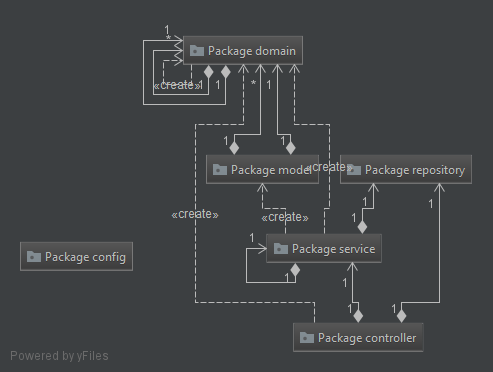
\includegraphics[scale=.8]{diag_architecture.png}
\caption{Vue d'ensemble}
\end{figure}

\begin{table}[h]
	\centering
	\def\arraystretch{1.4}
	\begin{tabular}{|l|l|l|}
		\hline
		\textbf{Package} & \textbf{Description}\\
		\hline
		\texttt{domain} & Contient l'ensemble des définitions des EJB\\
	  \hline
		\texttt{model} & Contient l'ensemble des modèle annexes utilisés\\
	  \hline
		\texttt{service} & Contient la définition des services\\
	  \hline
		\texttt{controller} & Contient le routing du projet par la définition des contrôleurs\\
	  \hline
		\texttt{repository} & Définition des repository (outils de simplification de communication des données)\\
	  \hline
	\end{tabular}
\end{table}

\section{Données}
Avant de commencer le développement il est strictement nécessaire de choisir un moyen de faire fonctionner un système de persistance, notamment en choisissant une base de données parmi différents types :
\begin{itemize}
\item NoSQL
\item SGBD
\item SQL
\item ...
\end{itemize}
\vspace*{0.5cm}
Une fois la base de données choisie il nous faut définir le modèle relationnel sur lequel nous baser, c'est-à-dire la composition de nos tables et du stockage des données.


\subsection{Initialisation de la Base de Données}
Une fois choisi PostgreSQL nous nous sommes attelé à l'élaboration d'une solution relationnelle dans le but de répondre au mieux au projet. La configuration par défaut que nous avons défini est :

\begin{table}[h]
	\centering
	\def\arraystretch{1.4}
	\begin{tabular}{|l|l|l|}
		\hline
		Nom d'utilisateur PostgreSQL & Mot de Passe & Nom Base de données\\
		\hline
		postgres & postgres & jeedb\\
	  \hline
	\end{tabular}
\end{table}

Grâce à l'utilisation de Spring il est très facile de changer ces paramètre, il suffit d'aller dans :\\
\texttt{src/main/resources/application.properties}\\
Dans ce fichier nous trouvons facilement l'url de connexion à la base de données, le nom d'utilisateur et également le mot de passe.

\subsection{Diagramme relationnel}
\begin{figure}[h]
\centering
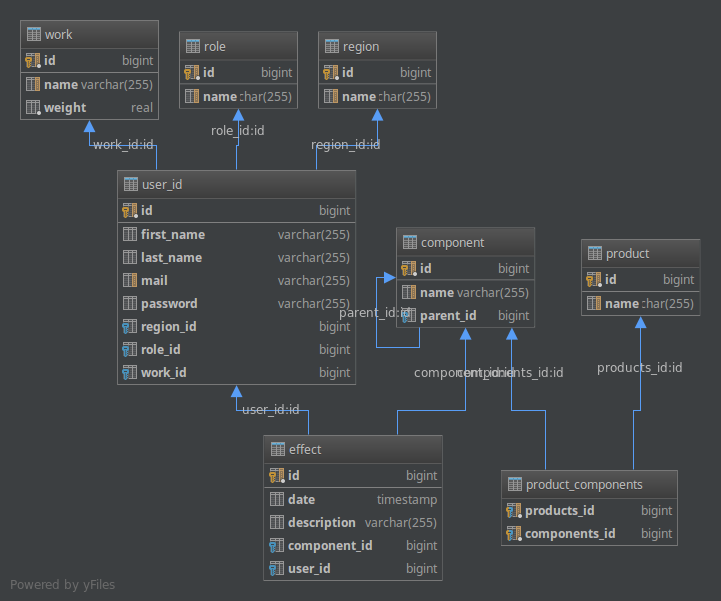
\includegraphics[scale=.55]{diag_bdd.png}
\caption{Diagramme Relationnel}
\end{figure}

\newpage

\vspace*{0.5cm}
\subsection{Liaison des Données}
Afin de faciliter la liaison de la couche données avec la couche métier nous avons utilisé l'API offerte par Spring : Spring-Data-JPA. En effet celle-ci vise à améliorer la mise en oeuvre de la couche d'accès aux données en réduisant considérablement l'effort d'écriture du code d'implémentation en particulier pour les méthodes CRUD et de recherche.\\
La notion centrale dans Spring-Data-JPA est la notion de Repository. Un repository est une interface à écrire par les développeurs. Cette interface requiert la déclaration des méthodes utiles d'accès aux données.

\vspace*{0.5cm}

\begin{figure}[h]
\centering
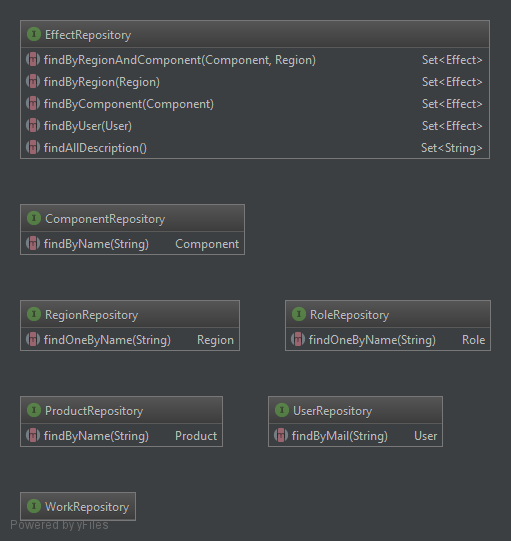
\includegraphics[scale=.8]{diag_repos.png}
\caption{Liste des différents Repository}
\end{figure}

\newpage

\vspace*{0.5cm}

Enfin, un exemple de déclaration de repository :

\begin{figure}[h]
\centering
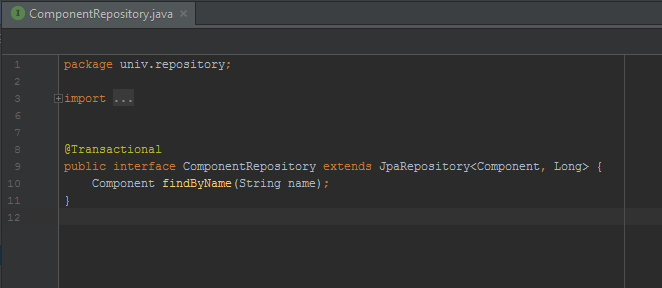
\includegraphics[scale=.8]{exemple_repos.png}
\caption{Exemple de Repository}
\end{figure}

\section{Les Entités}

\subsection{Description}
Dans un projet Spring, une entité se réfère étroitement à un entité que nous pourrions trouver dans un projet JavaEE natif. En effet nous privilégions les annotations dans le but de simplifier la lecture et l'affectation des tâches.

\begin{figure}[h]
\centering
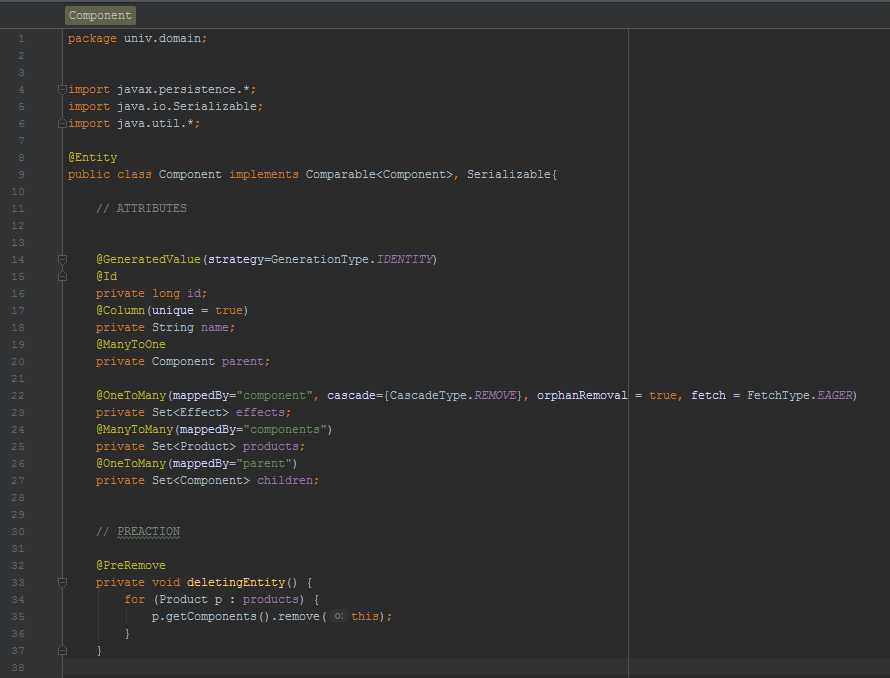
\includegraphics[scale=.56]{exemple_beans.png}
\caption{Exemple d'Entity}
\end{figure}

\newpage

\vspace*{0.5cm}

\subsection{Diagramme des EJB}
\begin{figure}[h]
\centering
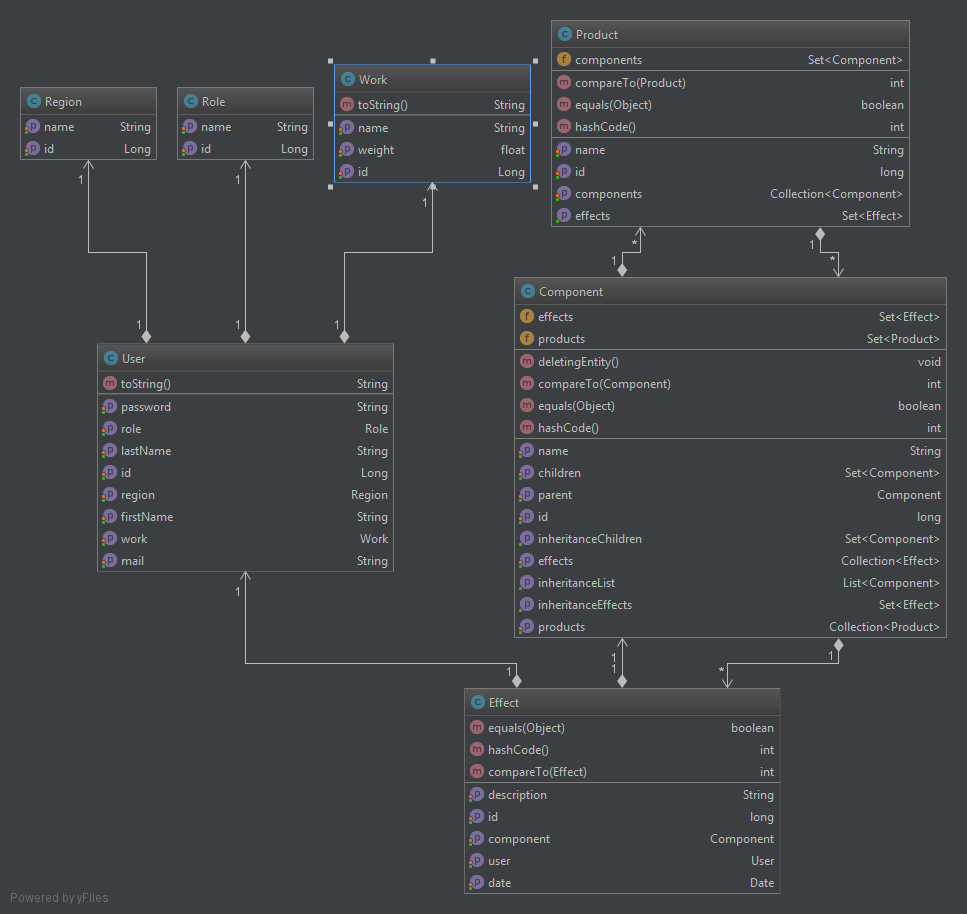
\includegraphics[scale=.4]{diag_beans.png}
\caption{Liste des différents Repository}
\end{figure}

\section{Services}
\subsection{Description}
Puisque nous sommes dans une Architecture Orientée Service, nous utilisons Spring afin de répondre à ce pré-requis. Dans cette couche, les services peuvent communiquer entre eux et permettre une meilleure productivité. Il faut noter que cette couche utilise les Repository dans le but de contextualiser convenablement les entités. Les services vont donc s'occuper de lier la couche métier avec la couche données dans le but de déclarer un contrat d'utilisation. Ce contrat permettra à nos contrôleurs de connaitre les conditions d'utilisation d'un service et de ne préoccuper que de sa définition.\\
Il est à noter également qu'un service à pour but d'être réutilisé par la suite et est donc prévu pour persister au-delà d'un unique projet, d'où l'intérêt de son utilisation.

\newpage

\vspace*{0.5cm}

\subsection{Diagramme de Services}
\begin{figure}[h]
\centering
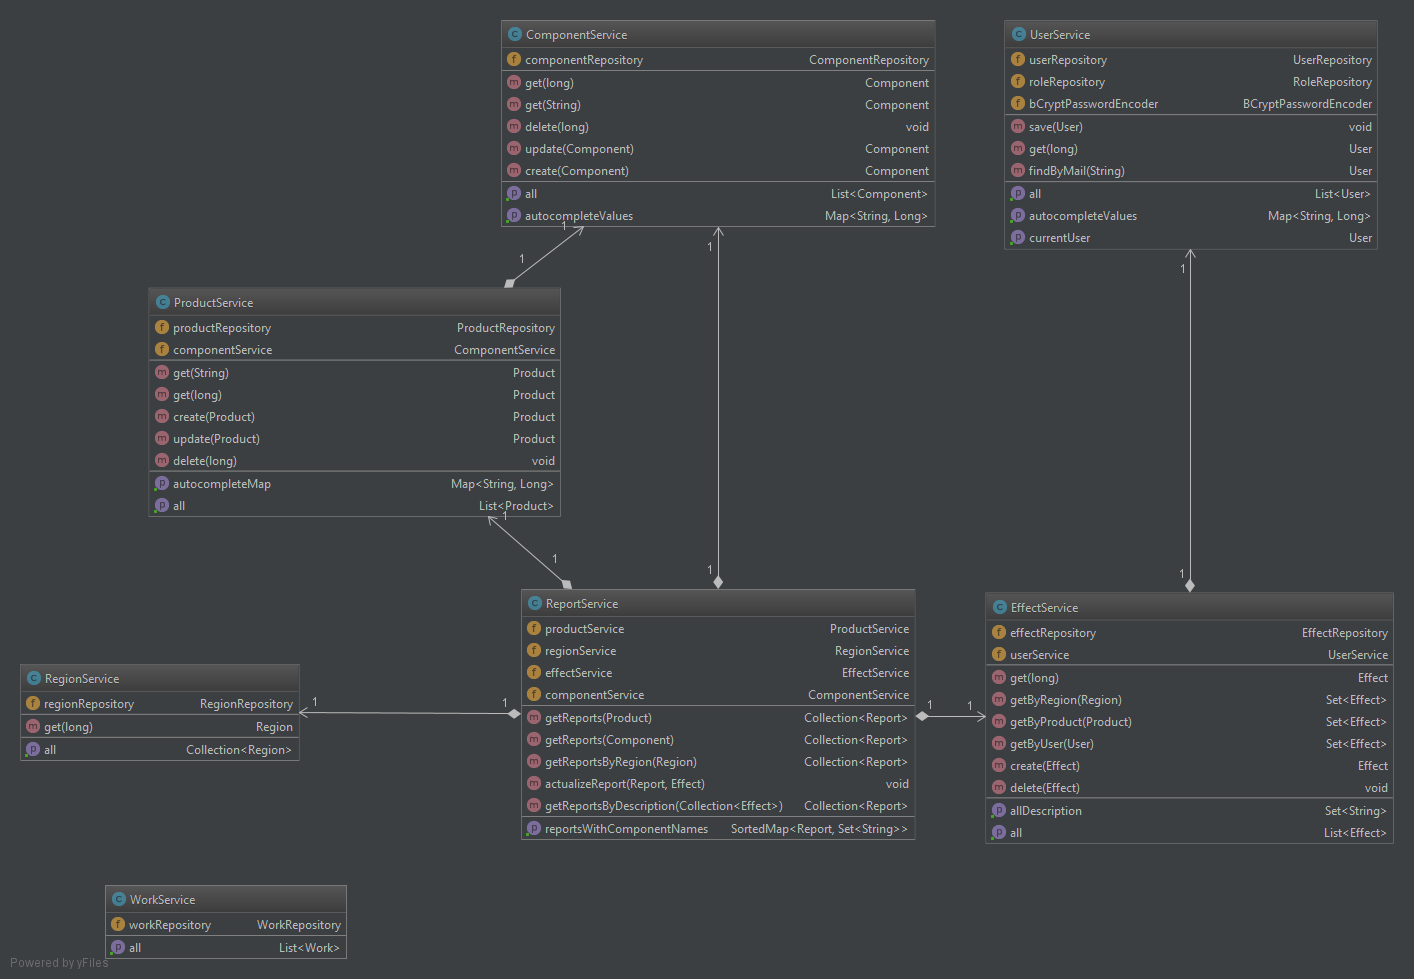
\includegraphics[scale=.3]{diag_service.png}
\caption{Liste des différents Repository}
\end{figure}

\section{Gestionnaire de sessions}
Dans le but de gérer la sécurité au sein de notre application nous avons décidé d'utiliser Spring Security. En effet celui-ci nous permet de rapidement contrôler les différentes authentifications et connexions. Grâce à un fichier de mapping et à la définition d'un fichier de configuration, nous pouvons rapidement et efficacement définir le contrat de sécurité de notre application.

\begin{figure}[h]
\centering
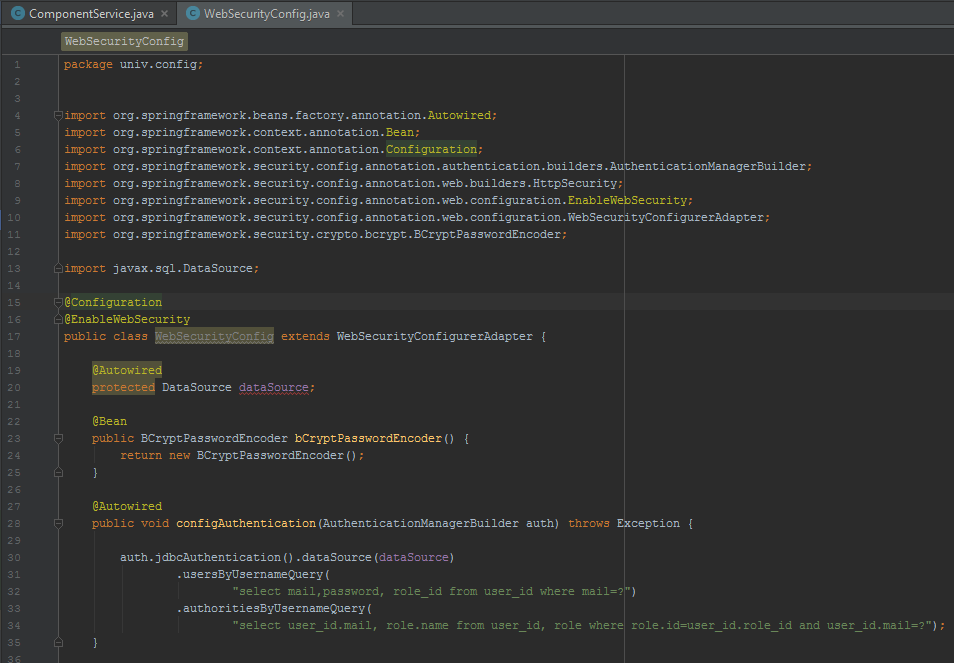
\includegraphics[scale=.3]{example_secur.png}
\caption{Liste des différents Repository}
\end{figure}

\end{document}